\documentclass{article}

% if you need to pass options to natbib, use, e.g.:
%     \PassOptionsToPackage{numbers, compress}{natbib}
% before loading neurips_2020

% ready for submission
% \usepackage{neurips_2020}

% to compile a preprint version, e.g., for submission to arXiv, add add the
% [preprint] option:
%     \usepackage[preprint]{neurips_2020}

% to compile a camera-ready version, add the [final] option, e.g.:
%     \usepackage[final]{neurips_2020}

% to avoid loading the natbib package, add option nonatbib:
\usepackage[nonatbib]{neurips_2020}
\usepackage{graphicx}
\usepackage[utf8]{inputenc} % allow utf-8 input
\usepackage[T1]{fontenc}    % use 8-bit T1 fonts
\usepackage{hyperref}       % hyperlinks
\usepackage{url}            % simple URL typesetting
\usepackage{booktabs}       % professional-quality tables
\usepackage{amsfonts}       % blackboard math symbols
\usepackage{nicefrac}       % compact symbols for 1/2, etc.
\usepackage{microtype}      % microtypography

\title{Project Report - ECE 176}

% The \author macro works with any number of authors. There are two commands
% used to separate the names and addresses of multiple authors: \And and \AND.
%
% Using \And between authors leaves it to LaTeX to determine where to break the
% lines. Using \AND forces a line break at that point. So, if LaTeX puts 3 of 4
% authors names on the first line, and the last on the second line, try using
% \AND instead of \And before the third author name.

\author{%
  Marco Paredes \\
  Electrical and Computer Engineering\\
  A15951023\\
}

\begin{document}

\maketitle

\begin{abstract}

    
    Enhanced Super-Resolution Generative Adversarial Networks (ESRGAN) are deep-convolutional GAN networks used for image super-resolution. It is an improved version of the state-of-the-art original SRGAN algorithm introduced in 2017 [1]. The ESRGAN is mostly composed of the original architecture of SRGAN but is composed of four major enhancements: batch norm removal, using features before VGG activation, relativistic discriminator, and a deeper network with RRDB. As seen on the original paper from ESRGAN and with the results on two different databases on this paper, ESRGAN performs better in being able to create high-resolution images. As also seen in the original research article, ESRGAN had a better performance than other models like RCAN, EDSR, and EnhanceNet. This paper will explore the ESRGAN results even further by collecting three different datasets and see how well the generator can perform in each dataset, including one with degraded (noisy) images. By doing so, the discriminator can be understood more by analyzing its ability to generalize its task on data it has not seen. 
    

\end{abstract}

\section{Introduction}
SRGAN networks have been shown to be effective in super-resolution, however, the outputs over-smoothed results without sufficient high-frequency details. As mentioned in the original ESRGAN paper, SRGAN uses the Peak Signal-to-Noise Ratio metric but fundamentally produces results that disagree with the subjective evaluation of human observers. In other words, the generated high-resolution images do not closely resemble what is seen in the ground truth picture. ESRGAN’s primary goal is to upscale low-resolution images while maintaining high-quality visual details. The algorithm is trained on GAN networks where it involved two main stages: first, the network’s generator is trained to produce an initial high-resolution image from a low-resolution input. Then, a discriminator network is introduced to assess the visual quality of the generated image and provides feedback to the generator network. Lastly, both the discriminator and the generator are updated based on the discriminator’s feedback to improve the image quality. ESRGAN employs other several CNN techniques to enhance image quality, including residual learning, to allow the network to learn the difference between low and high-resolution images more efficiently. In addition, the model uses VGG-19 networks to extract features from the generated images and the ground truth images and calculates the loss between them. 

Although the original paper [2], explores the results of the ESRGAN based on a celebrity dataset, we will further analyze the model and its results by training three different models, one for each dataset. The datasets will be the celebrity dataset, a popular dataset of dog images, and a dataset of degraded noisy pictures. For the celebrity and dog dataset, we will train a model for each and compare its results to see which model produced better, more realistic images. In addition, another model will be trained on the noisy dataset, which will be created by using the dog dataset and using NumPy functions to add an additional noise filter. 


\section{Related Work}
As mentioned before, the ESRGAN is an enhanced version of the state-of-the-art SRGAN model [1]. The SRGAN uses an architecture called SRResNet which is based on the concept of residual blocks. The generator consists of an initial convolutional layer, a series of residual blocks, and a series of upsampling layers followed by a final layer. It also uses a discriminator designed to distinguish between real high-resolution images and super-resolved images generated by the generator (the ESRGAN takes a step further to calculate the relativistic loss). The perceptual loss of the SRGAN is calculated as a combination of content loss, adversarial loss, and perceptual loss (which is calculated using features extracted from a pre-trained VGG19 model). As we will further explore, the ESRGAN improves all the aforementioned components and had a better performance which resulted in sharper, more realistic generated images.

The research behind ESRGAN was also further extended, the new improved model was named Real-ESRGAN [3]. Similar to ESRGAN, the Real-ESRGAN was designed to handle a wider variety of real-world, degraded images. It builds upon the ESRGAN and introduces several key improvements in terms of architecture and training strategy, including a modified RRDB (Residual in Residual Dense Block) network where it incorporates more dense connections between the layers within each residual block. Additionally, it uses a different discriminator known as the PatchGAN discriminator. The PatchGAN discriminator operates on smaller patches of the image instead of the entire image and allows the model to focus on local image features and textures, resulting in better perceptual quality. Finally, the Real-ESRGAN was trained on a more diverse dataset that includes images with several types of degradation such as noise and blur. Although the ESRGAN can output great results, the Real-ESRGAN is better suited for handling real-world degraded images and offers superior performance in terms of perceptual quality. This paper will focus specifically on the performance of the ESRGAN when introduced to a dataset with similar types of degradation the in the hopes that it will generalize better real-world images and result in improved performance.


\section{Method}
The main aim of the ESRGAN network is to improve the overall image and perceptual quality of the SRGAN architecture. This section will explain the detailed structure of the proposed method in the original ESRGAN research paper and will break down the formulations and how it was implemented into PyTorch.

The total loss for the generator is the following:
\[ L_G = L_{percep} + \lambda L_G^{Ra} + \eta L_1 \]

Where \(L_{percep}\) is the perceptual loss is the 1-norm distance between generated image and the ground-truth image. A more effective perceptual loss was calculated by the ESRGAN by constraining features before VGG activation rather than after activation (which was done in SRGAN). \(L_G^{Ra}\) is the adversarial loss for the generator: \(L_G^{Ra} = -\mathop{{}\mathbb{E}}_{x_r}[log(1 - D_{Ra}(x_r, x_f))] - \mathop{{}\mathbb{E}}_{x_f}[log(D_{Ra}(x_f, x_r))]\). The discriminator loss is defined as: \(L_D^{Ra} = -\mathop{{}\mathbb{E}}_{x_r}[log(D_{Ra}(x_r, x_f))] - \mathop{{}\mathbb{E}}_{x_f}[log(1 - D_{Ra}(x_f, x_r))]\), where \(D_{Ra}\) is the relativistic discriminator and: \(D_{Ra}(x_r, x_f) = \sigma (C(x_r) - \mathop{{}\mathbb{E}}[C(x_f)]\). The relativistic discriminator tries to predict that a real image \(x_r\) is a relatively more realistic than a fake one \(x_f\).

This paper specifically focuses on building an improved generator as well as a relativistic average discriminator loss function. The following diagrams are overviews of the generator and discriminator networks, we will go more in-depth about each important component:

\begin{center}
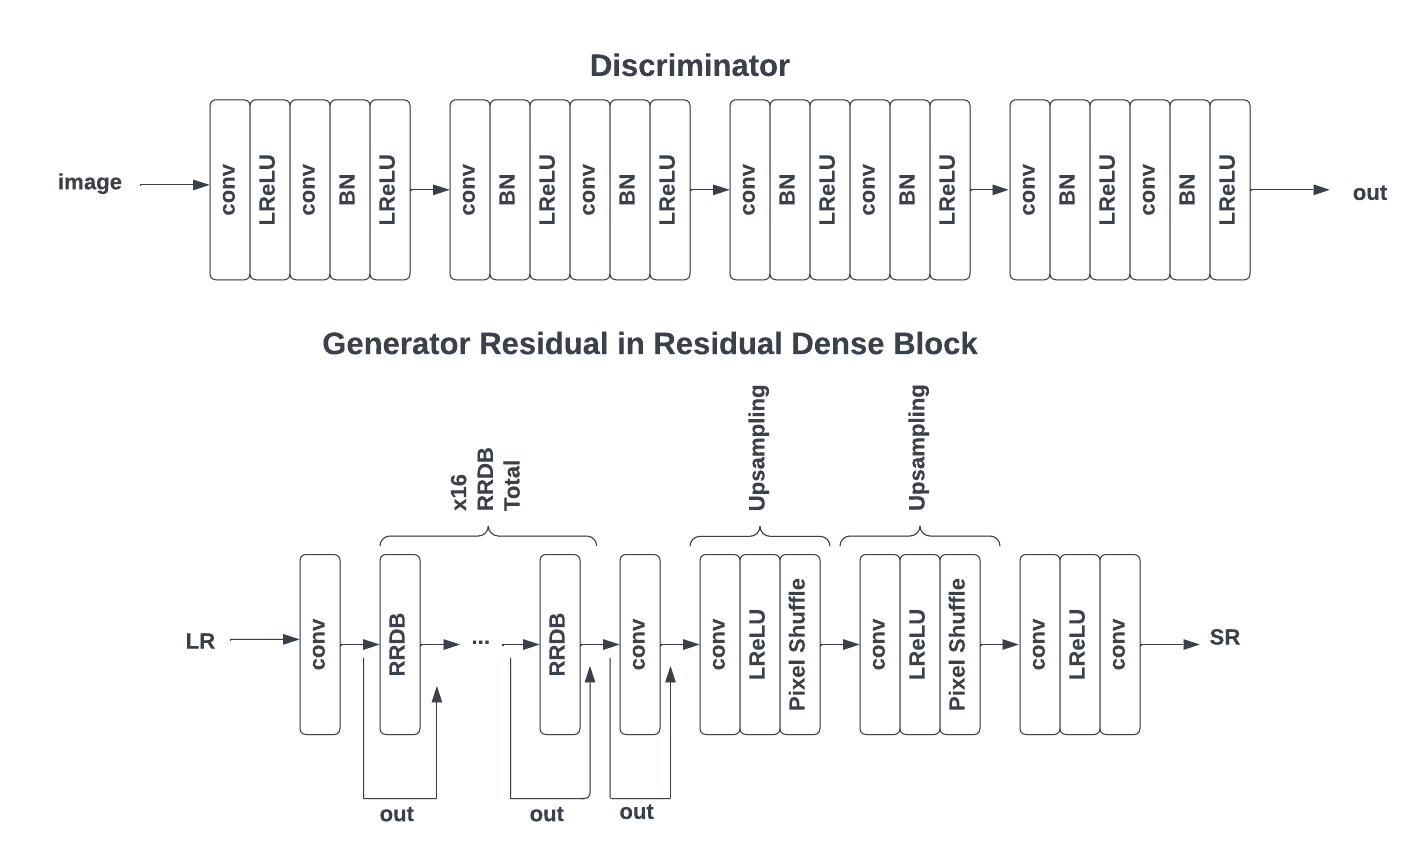
\includegraphics[scale=0.4]{images/discriminator_and_generator.png}
\end{center}

The Discriminator is composed of 23 total layers, and it is built on the previous discriminator network from SRGANs. The Generator is composed of 16 Residual in Residual Dense Blocks (which will be explained later) and two upsampling layers. As seen on the diagram, it is built from the fundamentals of ResNet blocks as the input of each layer is added onto its output. The Generator then contains two upsampling layers composed of a convolutional network, Leaky ReLU, and a Pixel Shuffle. All of this generates a single super-resolution image which is then used to compute the perceptual loss.

The following diagrams explain the structure behind the Residual in Residual Dense Block which is composed of three Dense Residual Blocks. Each Dense Residual Blocks output is added with its respective inputs. By using these blocks, the network can achieve improved gradient flow by enabling gradients to flow more easily through the network through backpropagation. It also helps facilitate the reuse of features across multiple layers, enabling the network to leverage both local and global features more effectively. By doing this, it allows for enhanced feature integration of low-level and high-level features. This can lead to better performance on tasks that required a combination of fine-grained details and high-level abstractions.

\begin{center}
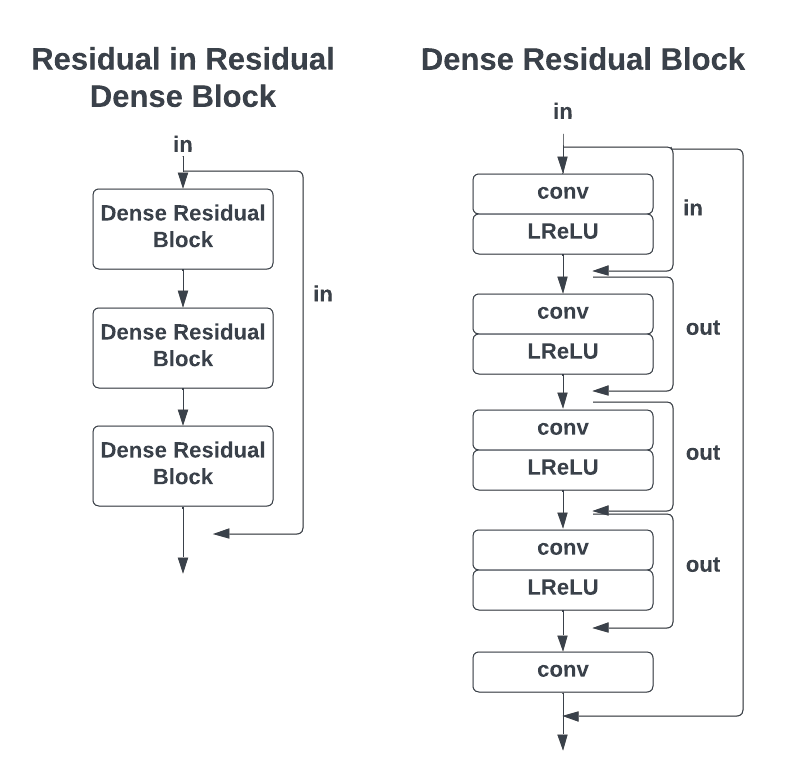
\includegraphics[scale=0.25]{images/rrdb.png}
\end{center}

The SRGAN network effectively uses residual blocks to add the input to each layer, however, the ESRGAN uses a denser residual network that effectively keeps track of fine-grained details that help create sharper images and therefore higher perceptual accuracy. 


\section{Experiments}

In this report, 3 different datasets were used. First, it is a celebrity dataset that was used by the original creators of the ESRGAN network [4]. This was used to check the training of the model and if it was working effectively. Since it is a very large dataset and there were little computation resources that could be used, the dataset was split into 1/128 its size, resulting in 1582 different images. Although it was very few images compared to the whole dataset, the generative model still proved effective in producing higher-quality images. Following is a random collection of images from the celebrity dataset:

\begin{center}
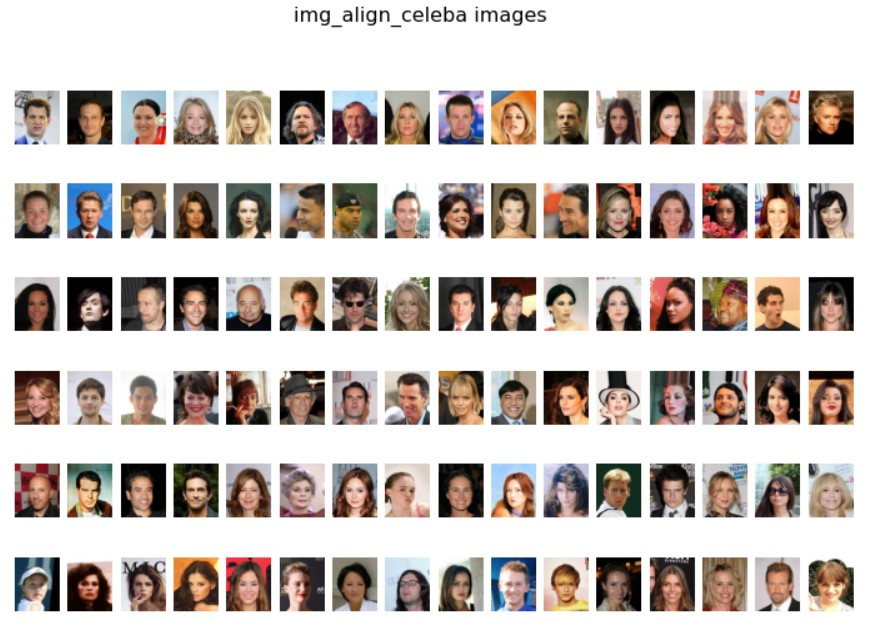
\includegraphics[scale=0.5]{images/img_align_celeba_images.jpg}
\end{center}

After the completion of the training, the generator produced the following images during training. The training iterated through 5 epochs with 791 batches each.

\begin{center}
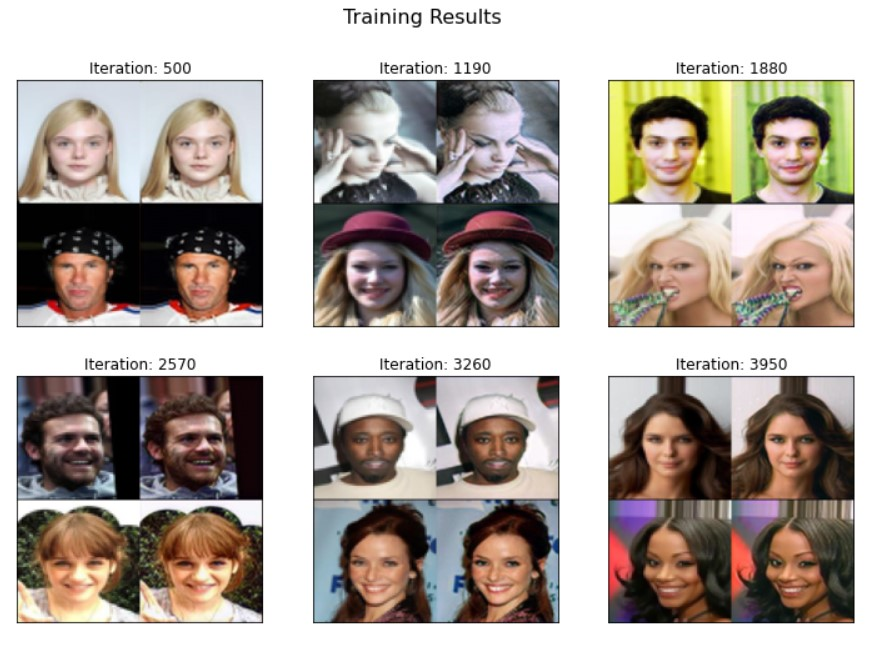
\includegraphics[scale=0.5]{images/img_align_celeba_training_results.jpg}
\end{center}

As seen above, the quality of the lower image resolution was improved. Compared to the original ESRGAN model in the research paper, they were able to produce much finer details as they had multiple GPUs at their disposal. Due to limited time and resources, not much training was done on the dataset above with this observed model. Either way, the results prove that the generator worked well. The next dataset was a dog dataset of different breeds [5]. The dataset was used to test the training of the model with new data and observe how well it did. Similar to the celebrity dataset, since there were too many images in this dataset, it was cut down to 1/8 of the original size. Following is a random collection of images from the dog dataset:

\begin{center}
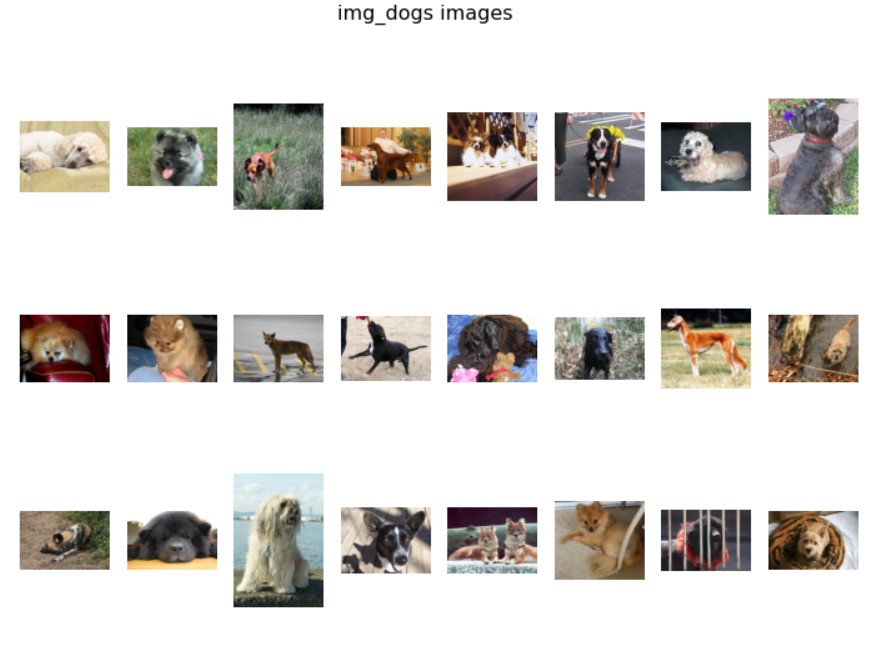
\includegraphics[scale=0.5]{images/img_dogs_images.jpg}
\end{center}

The generator and discriminator were both trained with 5 epochs and 1286 batches each. The best \(L_G\) loss for the generator was 1.08 while for the discriminator, the best loss \(L_D^{Ra}\) that was produced was 1.58e-08. From these values, the best generator and discriminator were saved. As seen, even with limited data and training, the generator was effective in being able to produce higher-quality images. If observed closely, more contrast and brightness were added to the pictures. These were likely from the high-level feature extraction from the VGG-19 as well as the Residual in Residual Dense Blocks. It was able to produce the following results:

\begin{center}
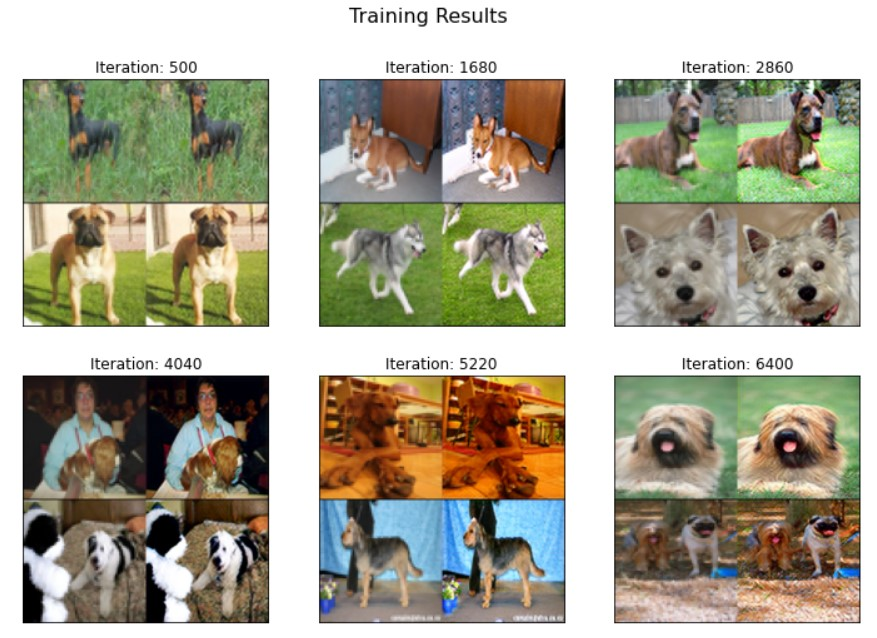
\includegraphics[scale=0.5]{images/img_dogs_training_results.jpg}
\end{center}

 Next, we are going to observe how the model will work when trained on a noisy dataset. In other words, the dog dataset was used to create a noisy dog dataset using the NumPy function np.random.normal. Most of the pictures were copied with an additional noise filter. If there were any RGB values in the noisy image results that were above 255, they set to 255 and vice versa for 0. Following is a random collection of noisy images:

\begin{center}
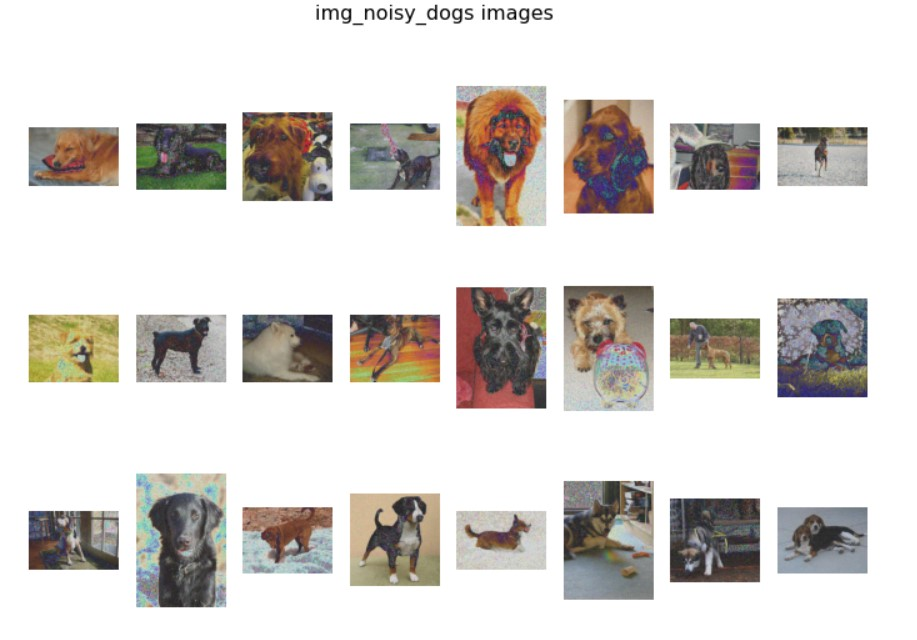
\includegraphics[scale=0.5]{images/img_noisy_dogs_images.jpg}
\end{center}

Finally, the model produced the following results:

\begin{center}
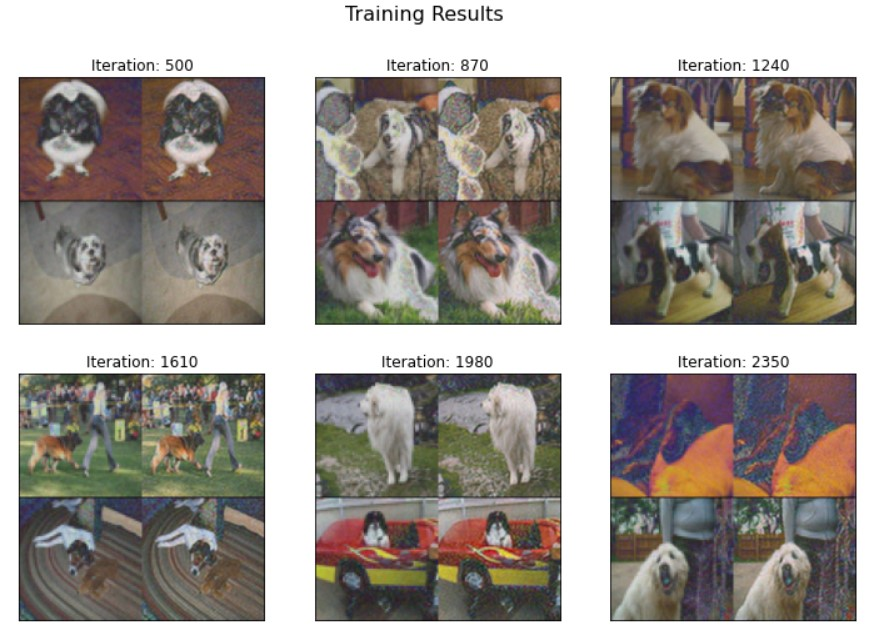
\includegraphics[scale=0.5]{images/img_noisy_dogs_training_results.jpg}
\end{center}

Compared to the previous models and results, unfortunately, the generator was not as effective in producing sharp high-quality images. There are a few instances, for example, observing the bottom pictures in iteration 870, where the generator produced higher-quality images but in those cases, the low-quality image did not have much noise. One possible reason why the training did not work as effectively, in this case, is that the model was trained on a blurred lower-quality version of the already added noise filter. In other words, the noisy filter was added to the images after the pictures were resized and made to lower quality. Due to that reason, the noise is not as visible in the low-resolution images on which the model was trained. 

In conclusion, the ESRGAN is effective in producing high-quality images from low-resolution inputs, even with minimal data and training. It would be interesting to see the results of the trained model with a larger dataset with more training and see how well it is able to generate high-quality pictures from the noisy ones. With that model too, it would be good to see how well the generator from the normal dog dataset is able to produce images from the noisy inputs. Given little training time, it is probable it would not be effective but would be a good analysis for a stronger model.

\section{Supplementary Material}

The code that was used to create the model was PyTorch and took inspiration from eriklindernoren's GitHub Repo "PyTorch-GAN" (it was not copied and pasted) [6]. They used the celebrity dataset that is used in this project and were able to produce fine results. They also have a number of other GAN networks that people could look into.

\section*{References}

\begin{enumerate}
  \item [1]: Ledig, Christian, et al. “Photo-Realistic Single Image Super-Resolution Using a Generative Adversarial Network.” ArXiv.org, 25 May 2017, https://arxiv.org/abs/1609.04802. 
  \item [2]: Wang, Xintao, et al. “Esrgan: Enhanced Super-Resolution Generative Adversarial Networks.” ArXiv.org, 17 Sept. 2018, https://arxiv.org/abs/1809.00219. 
  \item [3]: Wang, Xintao, et al. “Real-ESRGAN: Training Real-World Blind Super-Resolution with Pure Synthetic Data.” ArXiv.org, 17 Aug. 2021, https://arxiv.org/abs/2107.10833. 
  \item [4]: “Large-Scale Celebfaces Attributes (Celeba) Dataset.” CelebA Dataset, http://mmlab.ie.cuhk.edu.hk/projects/CelebA.html. 
  \item [5]: Khosla, Aditya, et al. Stanford Dogs Dataset, http://vision.stanford.edu/aditya86/ImageNetDogs/main.html. 
  \item [6]: Eriklindernoren. “Eriklindernoren/Pytorch-Gan: Pytorch Implementations of Generative Adversarial Networks.” GitHub, https://github.com/eriklindernoren/PyTorch-GAN. 
\end{enumerate}

\end{document}




